In this section, we want to motivate the advantage of the numerical smoothing idea in the context of MLMC method. For this aim we consider two examples: i) the first one is for computing the price of a digital option (see Section \ref{sec: MLMC for digital options}) , and ii) the second example is for approximating a density function (see Section \ref{sec: MLMC for approximating densities and greeks}). The idea and results of the first example can be generalized to i)  any kind of option having low regularity in the payoff function, or  ii) for computing distribution functions, since it involves the indicator function.  On the other hand, the second example have two important applications: i) computing density functions which involves the use of Dirac delta functions and which is hard to approximate its expectation using MLMC due to the infinite variance, and ii) computing Greeks for an option with a non smooth payoff function.
\subsection{Our contributions to the literature}
Usually, for such  tasks, standard MLMC will fail or not have the optimal performance, due to the singularity present in the delta or the indicator functions, implying either high variance or kurtosis for the MLMC estimator. In the literature, few works tried to address this issue. For instance,
\begin{enumerate}
\item Avikainen in \cite{avikainen2009irregular}, and Giles, Higham, and Mao in \cite{giles2009analysing} used MLMC for such a task without smoothing.
\item On the other hand, a second approach  was suggested in  \cite{giles2008improved,giles2013numerical}, that used implicit smoothing based on the use of conditional expectations. There are two potential issues  with this second approach: i) In general cases, one may have dynamics where it is not easy to derive an  analytic expression for the conditional expectation and ii) This approach used a higher order scheme, that is the Milstein scheme, to improve the strong order of convergence, and consequently the complexity of the MLMC estimator. Such a scheme becomes very computationally expensive for higher dimensional dynamics.
\item In \cite{giles2015multilevel}, the authors suggested a different approach based on parametric smoothing.  In fact, they carefully constructed a regularized version of the QoI, based on a 
regularization parameter that depends on the weak and strong convergence rates and also  the tolerance requirement.  This approach, despite offering better performance for the MLMC estimator and a better setting for theoretical analysis, it has the practical disadvantage consisting in the difficulty of generalizing it to cases where there is no prior knowledge of the the convergence rates (that is they need to be estimated numerically), and also for each error tolerance, a new  regularization parameter needs to be computed.
\end{enumerate}    

In this work, we address a similar problem and  propose an alternative approach that is  based on numerical smoothing. Our approach compared to previous mentioned works, has the following advantages
\begin{itemize}
\item It can be easily applied to cases where one can not apply analytic smoothing.
\item We obtain similar  rates of strong convergence and MLMC complexity  as in  \cite{giles2008improved,giles2013numerical}, without the need to use higher order schemes such as Milstein scheme.
\item Our approach is parameter free compared to that of  \cite{giles2015multilevel}. Therefore, in practice it is much easier to apply for any dynamics and QoI.
\end{itemize} 

\subsection{MLMC for digital options}\label{sec: MLMC for digital options}
In this section, we motivate the idea of using the numerical smoothing idea to compute option prices for non smooth payoff function. For illustration, we consider  the price of the digital option, that is we want to approximate
\begin{align}
\expt{g(X)}=\expt{\mathbf{1}_{X>K}},
\end{align}
where $K$ is the strike. 

Then, using similar idea introduced in Section \ref{sec:The discretized 1D Black-Scholes}, we can show that
\begin{align}
\expt{g(X)}&=\expt{\mathbf{1}_{X>K}}\nonumber\\
&=\expt{1-\Phi(y^\ast{K})},
\end{align}
where $y^\ast(K)$ is the kink location obtained by solving numerically $X(T; y^\ast(x), \mathbf{z}_{-1})$, $\mathbf{z}$ is the Gaussian random  vector used for Brownian bridge construction, and $\Phi$ is the cumulative Gaussian distribution function.

As an illustration, we choose the digital option of GBM asset with parameters: $S_0=K=100$, $T=1$, $r= 0$, and   $\sigma=0.2$, and we compare MLMC results with the original payoff function (without numerical smoothing), given by Figure \ref{fig:euler_digital_without_smoothing},  and MLMC results after applying our numerical smoothing idea, given by Figure \ref{fig:euler_digital_with_smoothing}. From these two Figures we have the following conclusions:
\begin{enumerate}
\item The numerical smoothing has improved the rate of strong convergence from $1/2$ (without smoothing) to $1$ after doing the numerical smoothing (compare both top left plots in Figures \ref{fig:euler_digital_without_smoothing} and Figure \ref{fig:euler_digital_with_smoothing}.
\item The numerical smoothing has also dropped significantly the kurtosis by a factor $100$, this is can be seen clearly by comparing the middle right plots in both Figures \ref{fig:euler_digital_without_smoothing} and Figure \ref{fig:euler_digital_with_smoothing}. We stress that this is an important improvement, since one needs $\Ordo{\kappa}$ samples  to obtain a reasonable estimate for the variance. For instance,  the standard deviation of the sample variance for a random variable $X$ with zero mean is approximately $\sqrt{(\kappa-1)/N} \expt{X^2}$ where the kurtosis $\kappa$ is defined as $\kappa = \frac{\expt{X^4}}{(\expt{X^2})^2}$.  
\item Finally, improving the strong error rate after using the numerical smoothing, resulted in an improvement of the complexity rate going from $TOL^{-2.5}$ for the case without smoothing to  $TOL^{-2} \abs{\log TOL}^2$, where $TOL$ is a prescribed tolerance, for the case where MLMC is coupled with numerical smoothing (compare the bottom right plots in Figures \ref{fig:euler_digital_without_smoothing} and \ref{fig:euler_digital_with_smoothing}).
\end{enumerate}

Although, for numerical illustration purpose, we just considered GBM dynamics, we emphasize that our approach can be extended in a straightforward manner to any kind of dynamics, since it is based on numerical smoothing based on solving a root finding problem. Furthermore, our approach can be easily extended to any low regular observable, $g$. For instance, this idea can be applied for approximating distribution functions involving the indicator function as the observable $g$. Finally, In all these possible extensions, we expect similar gains to be observed compared   to the case of using MLMC without smoothing.
\FloatBarrier
	\begin{figure}[h!]
\centering
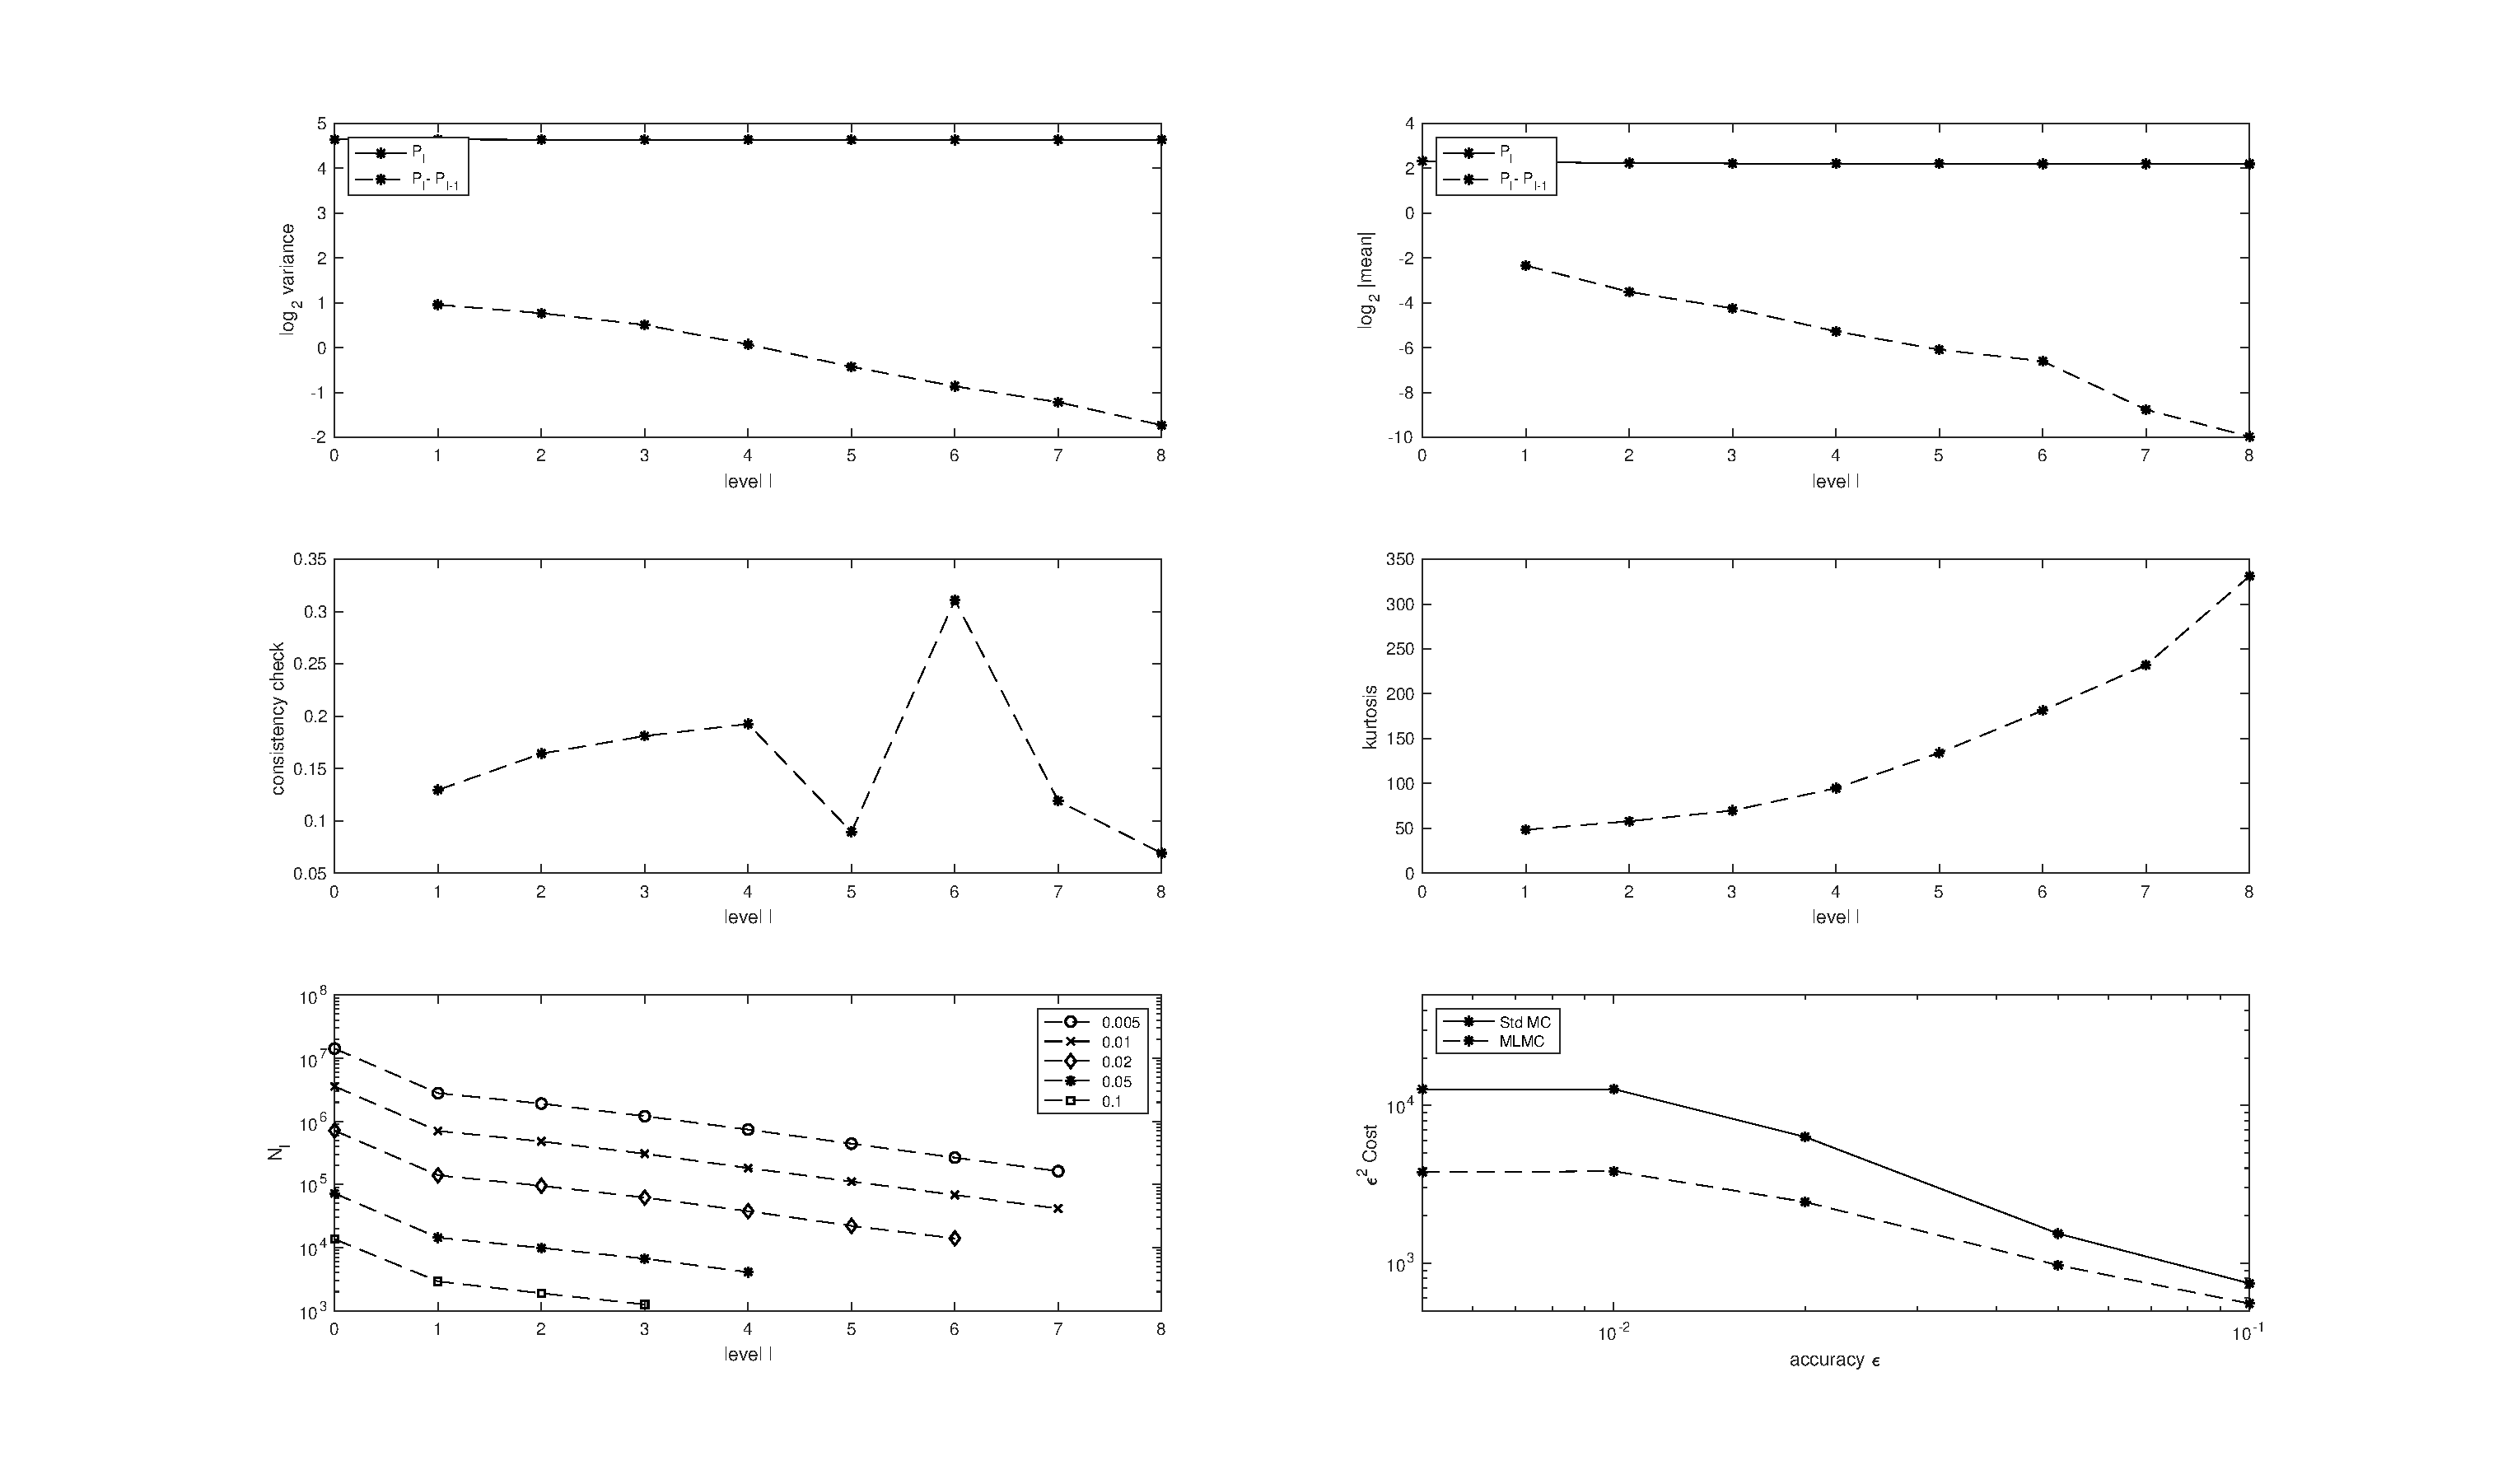
\includegraphics[width=0.7\linewidth]{./figures/MLMC_binary_opt/euler_digital_without_smoothing}

\caption{Numerical results for a digital call option using the MLMC method coupled with Euler-Maruyama discretisation of the GBM SDE, and without smoothing of the payoff.}
\label{fig:euler_digital_without_smoothing}
\end{figure}

\FloatBarrier
	\begin{figure}[h!]
\centering
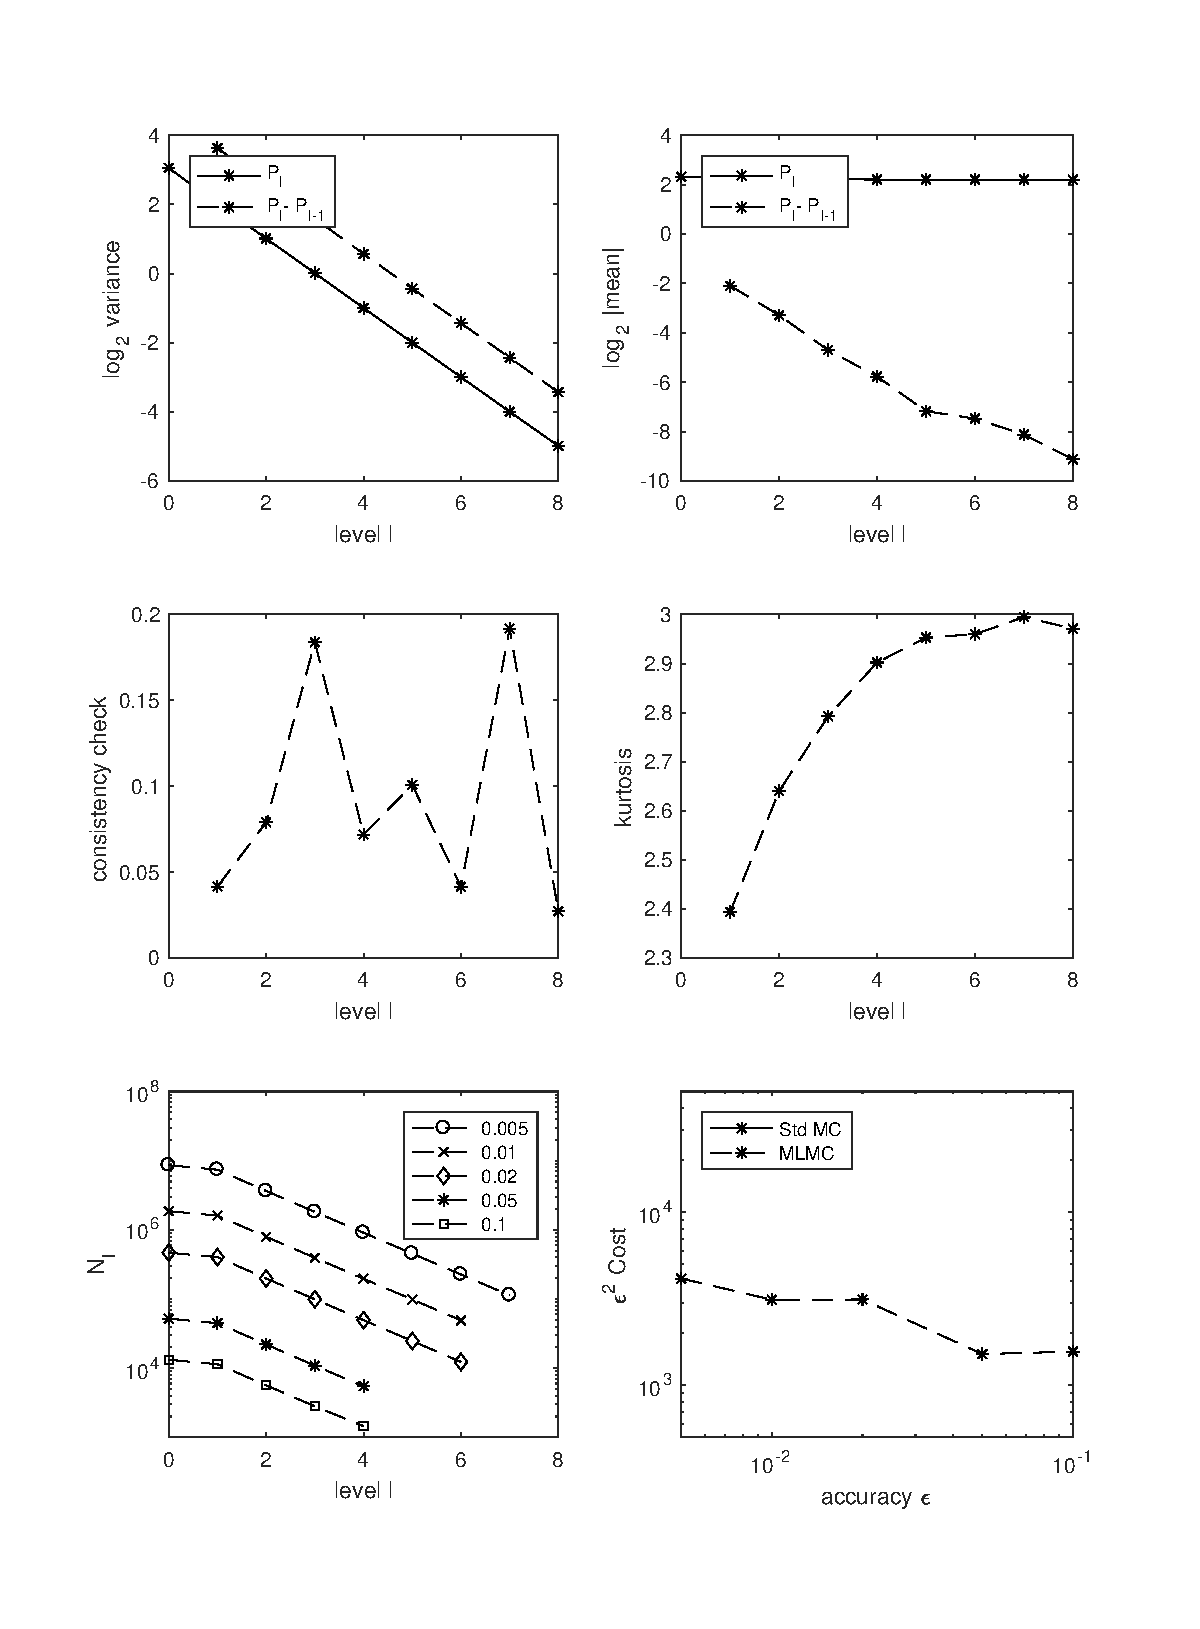
\includegraphics[width=0.7\linewidth]{./figures/MLMC_binary_opt/digital_option_with_smoothing_L_0_2_steps}

\caption{Numerical results for a digital call option using the MLMC method coupled with Euler-Maruyama discretisation of the GBM SDE, after applying  the numerical smoothing to the payoff. We mention that observing a decaying variance of $P_{\ell}$ here is expected since we used Brownian bridge for path construction, and the QoI depends only on the terminal value of the Brownian bridge which has a variance scaled of order $\Delta t$.}
\label{fig:euler_digital_with_smoothing}
\end{figure}

\FloatBarrier


\subsection{MLMC for approximating densities and Greeks}\label{sec: MLMC for approximating densities and greeks}
In this section, we motivate the idea of coupling the numerical smoothing  with MLMC method to compute density functions and Greeks for non smooth payoff functions. We remind that MLMC without any smoothing  will fail due to the infinite variance caused by the singularity of  the delta function. The aim in this case is to approximate the density, $\rho_{X}(u)$, for a given stochastic process $X$, at point $u$, and which is given by 
\begin{align}
\rho_{X}(u)=\expt{\delta(X-u)},
\end{align}
where $\delta$ is the Dirac delta function.

We can show that 
\begin{align}
\rho_{X}(u)&=\expt{\delta(X-y)}\nonumber\\
&=\exp\left(-(y^\ast(u))^2/2\right) \frac{d y^\ast}{dx}(u),
\end{align}
where $y^\ast(K)$ is the kink location obtained by solving numerically $X(T; y^\ast(x), \mathbf{z}_{-1})$, and $\mathbf{z}$ is the Gaussian random  vector used for Brownian bridge construction.


As an illustration, we choose to compute the density $\rho_{X}$  such that $X$ is a GBM with parameters: $S_0=K=1$, $T=1$, $r=0$, and $\sigma=0.2$. In this case, as a reference solution,  we know that $X(T)$ is lognormally distributed with parameters $r-\sigma^2$ and $\sigma^2$. In Figure \ref{fig:euler_density_MLMC_with_smoothing}, we show the numerical results  for computing the $\rho_{X}$ at $u=1$, using  MLMC coupled with the numerical smoothing idea. From Figure \ref{fig:euler_density_MLMC_with_smoothing}, we can check that we obtain a strong convergence rate of order $3/2$(see  top left plot in Figure \ref{fig:euler_density_MLMC_with_smoothing}), which results in a complexity of the MLMC estimator to be of order $TOL^{-2} \abs{\log TOL}^2$, where $TOL$ is a prescribed tolerance.

Although, for numerical illustration purpose, we just considered GBM dynamics, we emphasize that our approach can be extended in a straightforward manner to any kind of dynamics, since it is based on numerical smoothing based on solving a root finding problem. Furthermore, our approach can be easily extended to computing Greeks of a digital options, involving the delta functions.

\FloatBarrier
	\begin{figure}[h!]
\centering
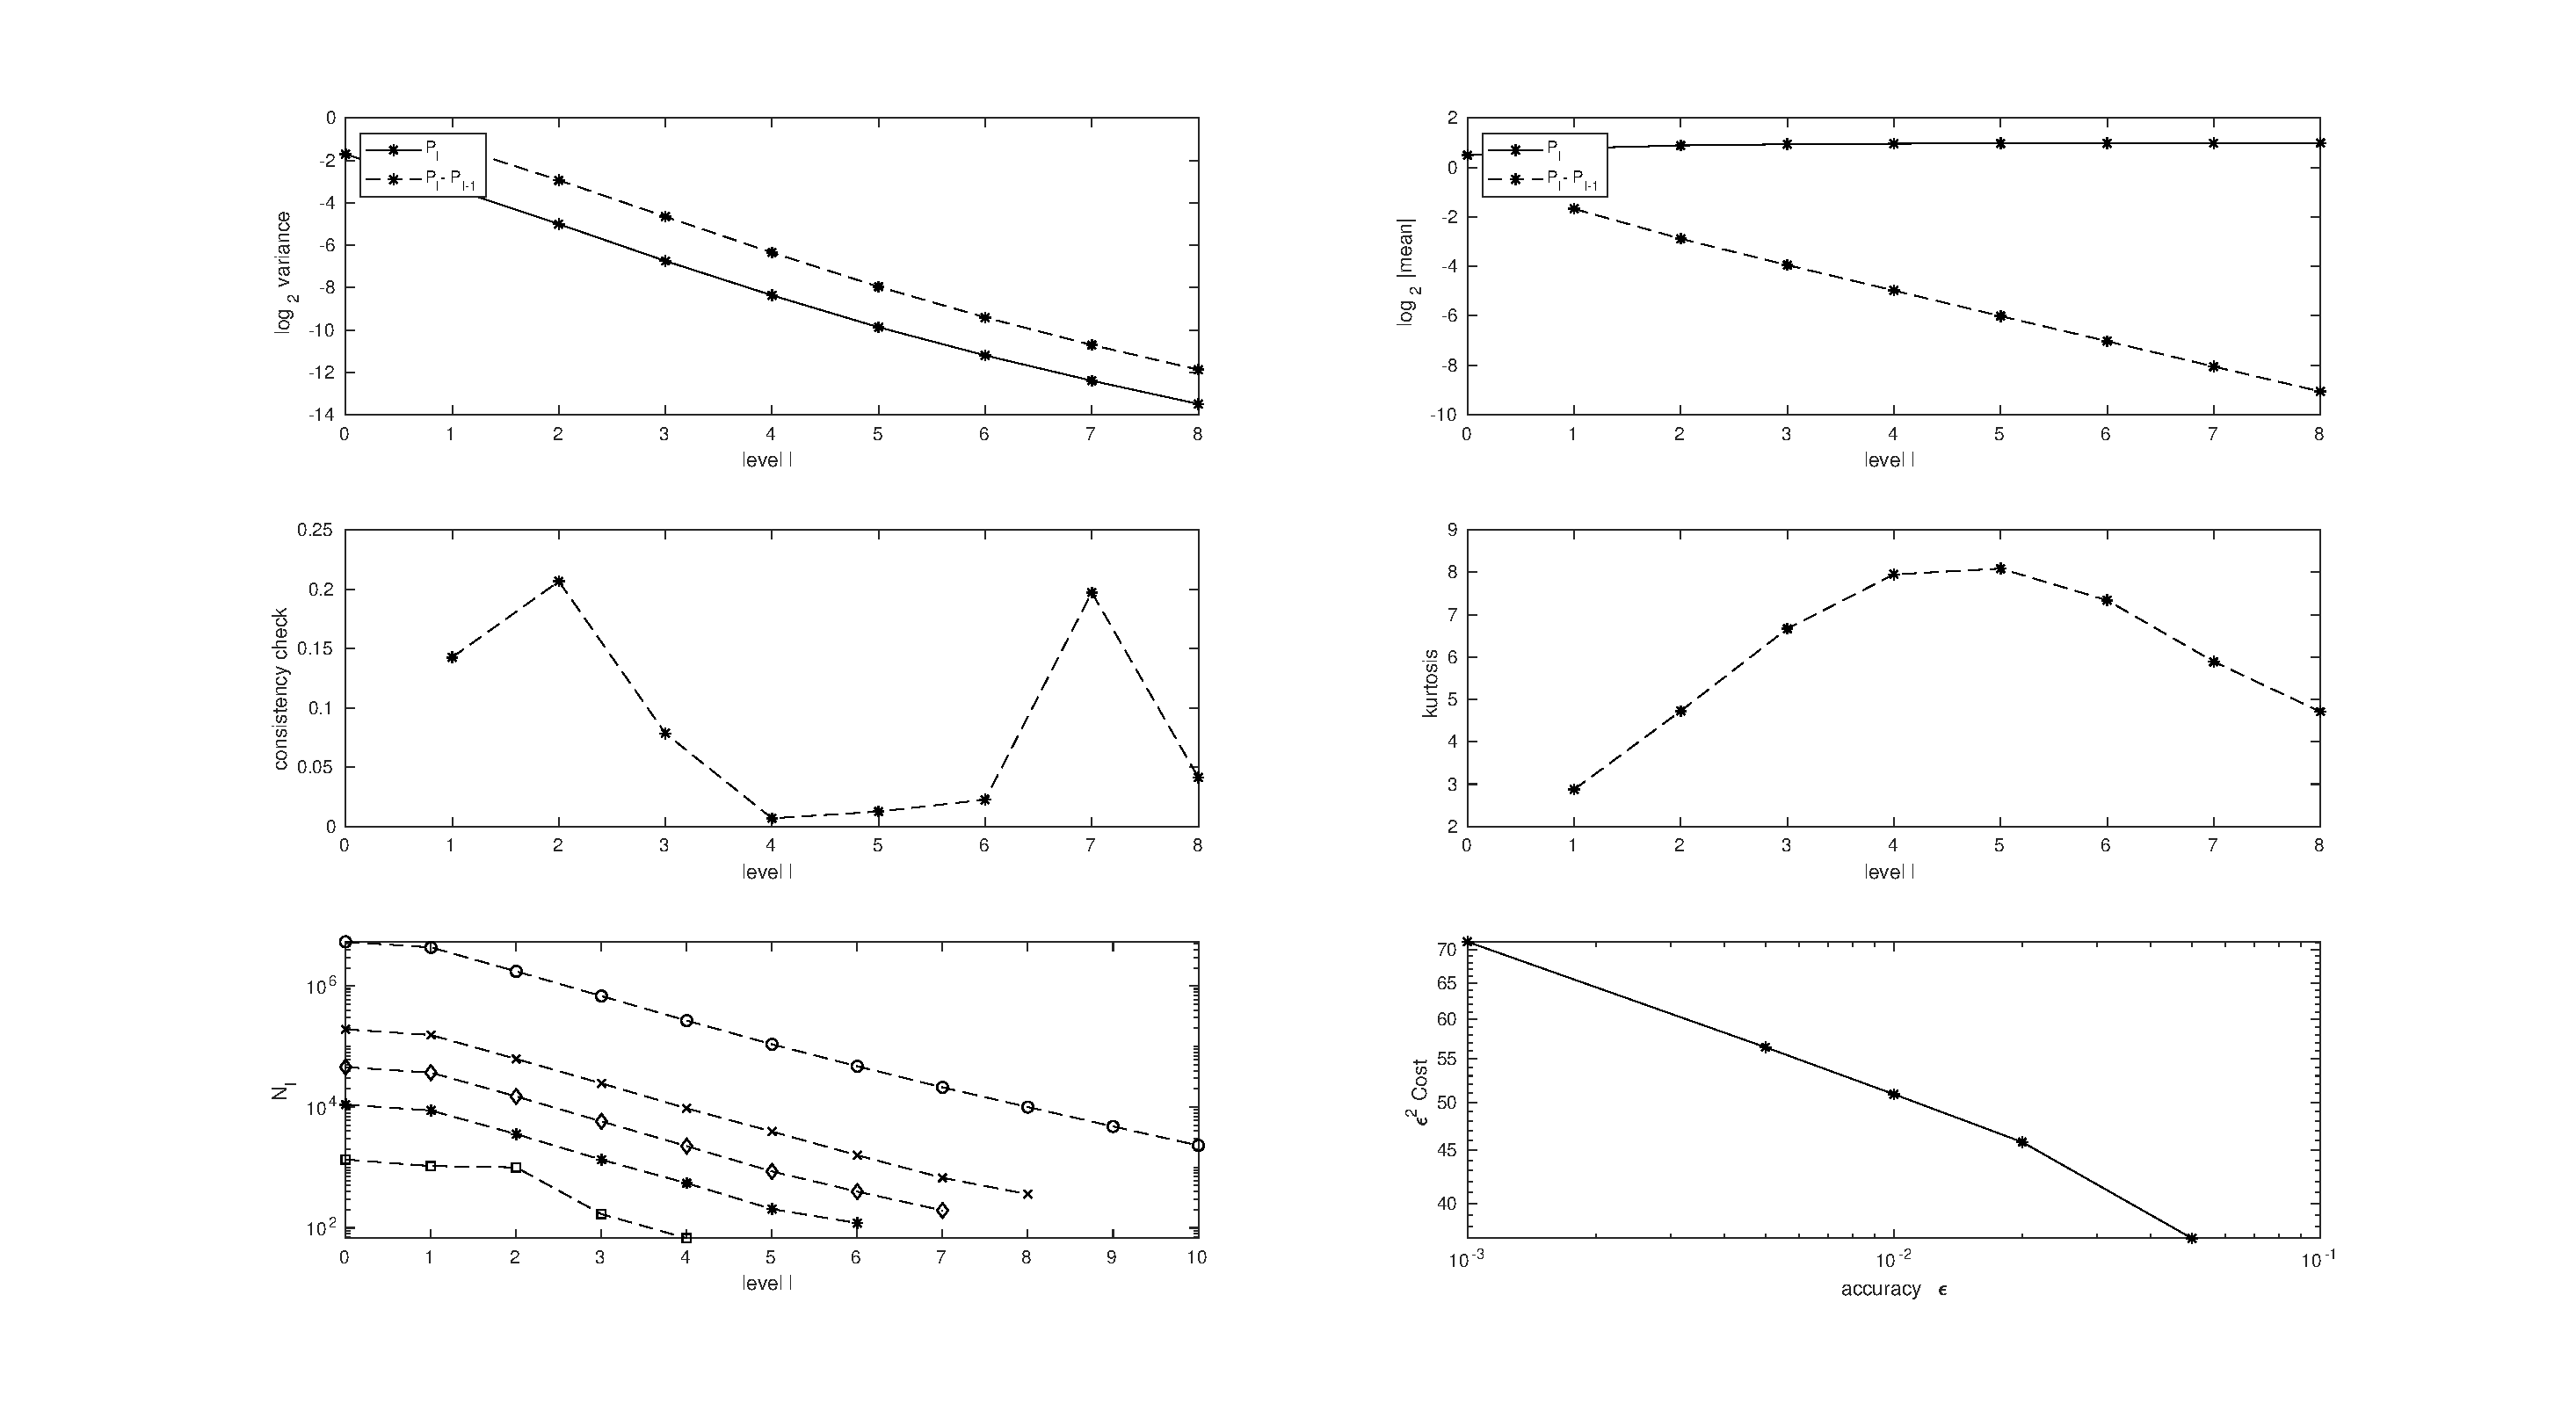
\includegraphics[width=1.0\linewidth]{./figures/MLMC_density_estimation/density_L0_1_L_8.eps}

\caption{Numerical results for  density estimation  using the MLMC method coupled with Euler-Maruyama discretisation of the GBM SDE, after applying  the numerical smoothing. We mention that observing a decaying variance of $P_{\ell}$ here is expected since we used Brownian bridge for path construction, and the QoI depends only on the terminal value of the Brownian bridge which has a variance scaled of order $\Delta t$.}
\label{fig:euler_density_MLMC_with_smoothing}
\end{figure}

\FloatBarrier

